\medskip

\subsection*{Partie A: Lectures graphiques}


\begin{enumerate}
\item Le nombre dérivé $f'(1)$ est égal au coefficient directeur de la tangente à $C_{f}$ au point $\mathrm{A}(1 ~;~ 2)$.

La tangente $T_{\mathrm{A}}$ passe par le point $\mathrm{C}(3 ~;~ 0)$ son coefficient directeur est donc égal à $\dfrac{0-2}{3-1}= \dfrac{-2}{2}=-1$.

Donc $f'(1)= - 1$.
\item  $f'(x)=0$ lorsque la tangente à la courbe est horizontale.

L'équation $f'(x)=0$ admet donc 2 solutions dans l'intervalle $]0 ~;~ 3]$ ce qui correspond à deux extremums de la fonction.
\item Graphiquement, sur l'intervalle $[0~;~0,5]$ le graphe de la fonction semble concave donc on en déduit :\quad $f''(0,2)~<~0$.
\end{enumerate}

\subsection*{ Partie B : Étude de la fonction \boldmath $f$\unboldmath}







\begin{enumerate}
\item $2X^{2}-3X + 2 = 0$ est une équation du second degré. Déterminons son discriminant~$\Delta$ :

$\Delta = (-3)^2-4 \times 2 \times 2 = 9-16=-7<0$

Le discriminant est négatif donc cette équation n'admet pas de solution sur $\R$.

$C_{f}$ coupe l'axe des abscisses à l'abscisse $x$ est équivalent à $f(x)=0$ soit

$x\left(2(\ln x)^{2}-3 \ln x+2\right)=~0$~.

Or $x >0$ donc $f(x)=0 \iff 2(\ln x)^{2}-3 \ln x+2 =0$

Posons pour $x > 0$, $X=\ln (x)$, l'équation devient : $2X^2-3X+2=0$  or on vient de démontrer que cette équation n'admet pas de solution sur $\R$ donc l'équation $f(x)=0$ n'admet pas de solution sur $\R$  donc  $C_{f}$ ne coupe pas l'axe des abscisses

	\item
	$f(x)=x\left(2(\ln x)^{2}-3 \ln x+2 \right)= x\left( \ln x\right)^2 \left( 2 - \dfrac{3}{\ln x}+\dfrac{2}{(\ln x)^2}\right)$.

	On sait  que $\lim\limits_{x\to +\infty }\ln x =+\infty$ donc $\lim\limits_{x\to +\infty }(\ln x)^2 =+\infty$

	d'où, d'une part : $\lim\limits_{x\to +\infty} x(\ln x)^2 = +\infty$

	et, d'autre part  $\begin{cases}  \lim\limits_{x \to +\infty }\frac{3}{\ln x} =0\\
		\lim\limits_{x\to +\infty } \frac{2}{(\ln x)^2}= 0\end{cases}$  donc, par somme $\lim\limits_{x \to +\infty } 2 - \dfrac{3}{\ln(x)}+\dfrac{2}{(\ln(x))^2} = 2$.

	Et finalement, par produit $\lim\limits_{x \to +\infty } f(x) =+\infty$.

\item
\begin{enumerate}
	\item $f'(x)=2(\ln x)^{2} + \ln x - 1$.
	
\emph{Non demandé} : $f$ est dérivable comme produit de sommes de fonctions de $x$ dérivables sur $]0~;~+ \infty[$ et sur cet intervalle :

$f'(x) = 2(\ln x)^2 - 3\ln x + 2 + x(4\ln x \times \dfrac 1x - 3\dfrac 1x) =  2(\ln x)^2 - 3\ln x + 2 + 4\ln x - 3  = 2(\ln x)^2 + \ln x - 1$.

On sait que $u$ étant une fonction de $x$ dérivable $\left(u^n\right)' = n u'u^{n-1}$

Donc pour tout $x$ appartenant à $]0~;~ +\infty[$:

$f''(x)= 2 \times 2 \ln x \times \dfrac{1}{x} + \dfrac{1}{x}-0 =\dfrac{1}{x}(4 \ln x + 1)$.

	\item Pour déterminer la convexité de $f$, déterminons le signe de $f''(x)$.

Sur $]0~;~+\infty[$, $\dfrac{1}{x} > 0$ donc $f''(x)$ est du signe de  $4 \ln x+1 $

$\begin{aligned} 4 \ln x+1 =0&  \iff \ln x = -\dfrac{1}{4}\\
	&\iff x = \e^{-\frac{1}{4}}
\end{aligned}$

$\begin{aligned} 4 \ln x+1 > 0& \iff \ln x > -\dfrac{1}{4}\\
			&\iff x > \e^{-\frac{1}{4}}
\end{aligned}$

Donc $f''(x) \geqslant 0 \iff x \in \left[\e^{-\frac{1}{4}}~;~+ \infty\right[$ : la fonction $f$ est convexe sur cet intervalle.

D'où :

\hfill~\begin{tikzpicture}
\tkzTabInit[lgt=3,espcl=3]{$x$/0.7,
	signe de $f''(x)$/0.7}{$0$,$\e^{-\frac{1}{4}}$,$+\infty$}
	\tkzTabLine{d,-,z,+,}
\end{tikzpicture}\hfill~

La fonction $f$ est concave sur  l'intervalle $\left]0~;~ \e^{-\frac{1}{4}}\right]$ et convexe sur l'intervalle $\left[ \e^{-\frac{1}{4}}~;~+\infty\right[$.

La valeur exacte de l'abscisse du point d'inflexion est $\e^{-\frac{1}{4}} \approx 0,779$.

		\item La fonction $f$ est convexe sur l'intervalle $\left[ \e^{-\frac{1}{4}}~;~+\infty\right[$
or $\e^{-\frac{1}{4}} <1$

donc la fonction $f$ est  convexe sur l'intervalle $[1~;~+\infty[$

et donc sur cet intervalle, la courbe $C_{f}$ est au-dessus de toutes ses tangentes, en particulier $T_{\mathrm{B}}$.
	\end{enumerate}
\end{enumerate}

\subsection*{Partie C : Calcul d'aire}

\begin{enumerate}
\item L'équation réduite de la tangente  $T_{\mathrm{B}}$ au point d'abscisse $\e$ est : $y= f'(\e)(x-\e )+ f(\e)$

$f'(\e)= 2(\ln \e)^{2} + \ln \e - 1 = 2 \times 1 + 1 - 1 = 2$ ;

$f(\e) = \e \left(2(\ln \e)^{2}-3 \ln e+2 \right)= \e \left(2 \times 1^2- 3 + 2\right)=  \e\times 1= \e$. (Ceci est dans l'énoncé mais pas clairement !)

La tangente $T_{\mathrm{B}}$ a donc pour équation réduite $y=2 x-\e$.

	\item $x \longmapsto x \ln x$ est de la forme $u v'$ avec $\begin{cases}u(x)=\ln x \quad\text { et }  \quad u'(x)=\frac{1}{x} \\ v'(x)=x \quad\text { et } \quad v(x)=\frac{x^2}{2}\end{cases}$

Les fonctions $u$ et $v$ sont continues car dérivables sur $\left[1~;~\e\right]$ et les fonctions $u'$ et $v'$ sont continues sur $\left[1~;~\e\right]$, donc, d'après la formule d'intégration par parties :

$\displaystyle \int_{a}^{b} u(x)v'(x)\, \mathrm{d}x = \Big [u(x)v(x)\strut\Big]_{a}^{b} - \int_{a}^{b} u'(x)v(x) \, \mathrm{d}x$.

d'où
$\begin{aligned}[t]
	\int_1^{\e}  x\ln x  \, \mathrm{d}x& =\Big[\ln x \times \dfrac{x^2}{2} \Big]_1^{\e}-\int_1^{\e} \left[\dfrac{1}{x} \times \dfrac{x^2}{2}\right] \, \mathrm{d}x\\
	& = \left( \ln \e \times \dfrac{\e^2}{2} \right) -\left(\ln 1 \times \dfrac{1^2}{2}\right) - \int_1^{\e} \dfrac{x}{2} \, \mathrm{d}x\\
	& = 1 \times \dfrac{\e^2}{2}- 0 - \Big[ \dfrac{x^2}{4} \Big]_1^{\e}\\
	& = \dfrac{\e^2}{2} - \left(\dfrac{\e^2}{4}-\dfrac{1}{4} \right)\\
	&= \dfrac{2\e^2}{4}- \dfrac{\e^2}{4}+\dfrac{1}{4} \\
	&= \dfrac{\e^{2}+1}{4}
\end{aligned}$




	\item On note $\mathcal{A}$ l'aire du domaine hachuré sur la figure, délimité par la courbe $C_{f}$, la tangente $T_{\mathrm{B}}$, et les droites d'équation $x=1$ et $x=\e$.

	Sur l'intervalle  $[1~;~\e]$, la courbe $C_{f}$ est au-dessus de la tangente $T_{\mathrm{B}}$ donc  l'aire du domaine hachuré sur la figure, délimité par la courbe $C_{f}$, la tangente $T_{\mathrm{B}}$, et les droites d'équation $x=1$ et $x= \e$ est égale, en unité d'aires,  à $\displaystyle \int_{1}^{\e} [f(x)-2x+\e ]~\mathrm{d} x$.

	$\begin{aligned}  \mathcal{A} &= \int_{1}^{\e} [f(x)-2x+\e] ~\mathrm{d} x\\
		&= \int_{1}^{\e} [2x(\ln x)^{2}-3x \ln x+2x -2x+\e] ~\mathrm{d} x\\
		&= 2\int_{1}^{\e} x(\ln x)^{2} ~\mathrm{d} x-3 \int_{1}^{\e} x \ln x ~\mathrm{d} x+ \int_{1}^{\e} \e  ~\mathrm{d} x \quad \text {par linéarité de l'intégrale}\\
		&= 2 \times \dfrac{\e^{2}-1}{4} - 3 \times \dfrac{\e^{2}+1}{4} + \Big[ \e x\Big]_1^{\e}\\
		&= \dfrac{2\e^2-2-3\e^2-3}{4} + \e^2-\e \\
		&= \dfrac{-\e^2-5}{4} +\dfrac{ 4\e^2-4\e}{4} \\
		&= \dfrac{3\e^2-5-4\e}{4}.\\
	\end{aligned}$.

Soit une aire d'environ 1,57 unités d'aire.

La valeur exacte de $\mathcal{A}$ est $\dfrac{3\e^2-4\e -5}{4} \,\rm{u.a.}$
\end{enumerate}

\medskip
